We begin by defining a formal model for describing surveillance strategy synthesis problems, in the form of a two player game between an agent and a target, in which the agent has only partial information about the target's location.

\subsection{Surveillance Game Structures}\label{sec:surveillance-games}
We define a \emph{surveillance game structure} to be  a tuple $G  = (\states,s^\init,\trans,\vis)$, with the following components:
\begin{itemize}
\item $\states = L_a \times L_t$ is the set of states, with $L_a$ the set of locations of the agent and $L_t$ the locations of the target;
\item $s^\init = (l_a^\init,l_t^\init)$ is the initial state;
\item $\trans \subseteq \states \times \states$ is the transition relation describing the possible moves of the agent and the target;
\item $\vis : \states \to \bools$ is a function that maps a state $(l_a,l_t)$ to $\true$ iff \emph{ position $l_t$ is in the area of sight of $l_a$}.
\end{itemize}


\begin{figure}
\subfloat[Surveilance arena \label{simple-grid}]{
%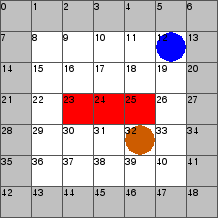
\includegraphics[scale=.33]{figs/7x7_safety.png}
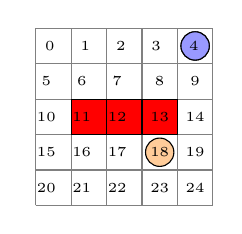
\begin{tikzpicture}[scale=0.9]
\draw[step=0.5cm,color=gray] (-1.5,-1.5) grid (1,1);
\filldraw[fill=blue,draw=black] (+0.75,+0.75) circle (0.2cm);
\filldraw[fill=red,draw=black] (0,0) rectangle (-0.5,-0.5);
\filldraw[fill=red,draw=black] (-0.5,0) rectangle (-1,-0.5);
\filldraw[fill=red,draw=black] (0,0) rectangle (0.5,-0.5);
\filldraw[fill=blue!40!white,draw=black] (+0.75,+0.75) circle (0.2cm);
\filldraw[fill=orange!40!white,draw=black] (0.25,-0.75) circle (0.2cm);
\node at (-1.30,+0.75) {\tiny{0}};
\node at (-0.80,+0.75) {\tiny{1}};
\node at (-0.30,+0.75) {\tiny{2}};
\node at (0.20,+0.75) {\tiny{3}};
\node at (0.73,+0.75) {\tiny{4}};
\node at (-1.35,+0.25) {\tiny{5}};
\node at (-0.85,+0.25) {\tiny{6}};
\node at (-0.35,+0.25) {\tiny{7}};
\node at (0.25,+0.25) {\tiny{8}};
\node at (0.75,+0.25) {\tiny{9}};
\node at (-1.35,-0.25) {\tiny{10}};
\node at (-0.85,-0.25) {\tiny{11}};
\node at (-0.35,-0.25) {\tiny{12}};
\node at (0.25,-0.25) {\tiny{13}};
\node at (0.75,-0.25) {\tiny{14}};
\node at (-1.35,-0.75) {\tiny{15}};
\node at (-0.85,-0.75) {\tiny{16}};
\node at (-0.35,-0.75) {\tiny{17}};
\node at (0.25,-0.75) {\tiny{18}};
\node at (0.75,-0.75) {\tiny{19}};
\node at (-1.35,-1.25) {\tiny{20}};
\node at (-0.85,-1.25) {\tiny{21}};
\node at (-0.35,-1.25) {\tiny{22}};
\node at (0.25,-1.25) {\tiny{23}};
\node at (0.75,-1.25) {\tiny{24}};
\end{tikzpicture}
}
\hfill
\subfloat[Transitions from the initial state\label{fig:simple-transitions}]{
\begin{minipage}{5.0cm}
\vspace{-1.8cm}
{\fontsize{8}{10}\selectfont $\vis(4,18) = \false,\vis(4,17) = \false,$ $\vis(4,19) = \true, \vis(4,23) = \false$}

\smallskip

\begin{tikzpicture}[node distance=.75 cm,auto,>=latex',line join=bevel,transform shape,scale=0.75]
\node at (0,0) (s0) {$(4,18)$};
\node  [below left of=s0,yshift=-.5cm] (s3) {$(3,23)$};
\node  [below right of=s0,yshift=-.5cm] (s4) {$(9,17)$};
\node  [left of=s3,xshift=-.35cm] (s2) {$(3,19)$};
\node  [left of=s2,xshift=-.35cm] (s1) {$(3,17)$};
\node  [right of=s4,xshift=.35cm] (s5) {$(9,19)$};
\node  [right of=s5,xshift=.35cm] (s6) {$(9,23)$};

\draw [->] (s0) edge (s1.north);
\draw [->] (s0) edge (s2.north);
\draw [->] (s0) edge (s3.north);
\draw [->] (s0) edge (s4.north);
\draw [->] (s0) edge (s5.north);
\draw [->] (s0) edge (s6.north);
\end{tikzpicture}
\end{minipage}

}
\caption{A simple surveillance game on a grid arena. Obstacles are shown in red, the agent and the target are coloured in blue and orange respectively.}
\label{fig:simple-surveillance-game}
\end{figure}

The transition relation $T$ encodes the one-step move of both the target and the agent, where the target moves first and the agent moves second. For a state $(l_a,l_t)$ we denote with $\succs_t(l_a,l_t)$ the set of successor locations of the target:

$\succs_t(l_a,l_t) = \{l_t' \in L_t \mid \exists l_a'. ((l_a,l_t),(l_a',l_t')) \in T\}$.

We extend $\succs_t$ to sets of locations of the target by stipulating that the set $\post(l_a,L)$ consists of all possible successor locations of the target for states in $\{l_a\} \times L$. Formally, let $\post(l_a, L) = \bigcup_{l_t \in L}\succs_t(l_a,l_t)$.

For a state $(l_a,l_t)$ and a successor location of the target $l_t'$, we denote with $\succs_t(l_a,l_t,l_t')$ the set of successor locations of the agent, given that the target moves to $l_t'$: 

$\succs_a(l_a,l_t,l_t') = \{l_a' \in L_a \mid  ((l_a,l_t),(l_a',l_t')) \in T\}$.

We assume that for every $s \in \states$ there exists $s' \in \states$ such that $(s,s') \in T$, that is, from every state there is at least one move possible (this might be staying in the same state).

We also assume that when the target moves to an invisible location, its position does not influence the possible one-step moves of the agent. Formally, we require that if $\vis(l_a,l_t') = \vis(l_a,l_t'')=\false$, then $\succs_a(l_a,l_t,l_t') = \succs_a(l_a,l_t,l_t'')$. This assumption is natural in the setting when the agent can move in one step only to locations that are in its sight.

\begin{example}\label{ex:simple-surveillance-game}
Figure~\ref{fig:simple-surveillance-game} shows an example of a surveillance game on a grid.  The sets of possible locations $L_a$ and $L_t$ for the agent and the target both consist of the squares of the  grid. The transition relation $T$ encodes the possible one-step moves of both the agent and the target on the grid, and incorporates all desired constraints. For example, moving to an occupied location, or an obstacle, is not allowed. Figure~\ref{fig:simple-transitions} shows the possible transitions from the initial state $(4,18)$.

The function $\vis$ encodes straight-line visibility: a location $l_t$ is visible from a location $l_a$ if there is no obstacle on the straight line between them. Initially the target is not in the area of sight of the agent, but the agent knows the initial position of the target. However, once the target moves to one of the locations reachable in one step, in this case, locations $\{17,19,23\}$, this might no longer be the case. More precisely, if the target moves to location $19$, then the agent observes its location, but if it moves to one of the others, then the agent no longer knows its exact location. \qed
\end{example}




\subsection{Belief-Set Game Structures}

In surveillance strategy synthesis we need to state properties of, and reason about, the information which the agent has, i.e. its \emph{belief} about the location of the target. To this end, we can employ a powerset construction which is commonly used to transform a partial-information game into a perfect information one, by explicitly tracking the knowledge one player has as a set of possible states of the other player.

For a surveillance game structure $G  = (\states,s^\init,\trans,\vis)$ we define the corresponding \emph{belief-set game structure} $G_\belief  = (\states_\belief,s^\init_\belief,\trans_\belief)$ with the following components:
\begin{itemize}
\item $\states_\belief = L_a \times \beliefs$ is the set of states, with $L_a$ the set of locations of the agent, and $\beliefs$ the set of \emph{belief sets} describing information about the location of the target;
\item $s^\init_\belief = (l_a^\init,\{l_t^\init\})$ is the initial state;
\item $\trans_\belief \subseteq \states_\belief \times \states_\belief$ is the transition relation where $((l_a, B_t),(l_a', B_t')) \in \trans_\belief$ iff one of these holds:
\begin{itemize}
\item[(1)] $B_t' = \{l_t'\}$, $l_t' \in \post(l_a,B_t)$, $\vis(l_a,l_t') = \true$;
\item[(2)] $B_t' = \{l_t' \in \post(l_a,B_t)  \mid  \vis(l_a,l_t') = \false \}$.
%\item[(1)] $B_t' = \{l_t'\}$ for some $l_t'$ such that $\vis(l_a,l_t') = \true$ and
%there exists $l_t \in B_t$ with $((l_a,l_t),(l_a',l_t')) \in \trans$;
%\item[(2)] $\begin{array}{lll}
%B_t' = \{l_t' & \mid & \vis(l_a,l_t') = \false \text{ and } \\
%&& \exists l_t \in B_t.\ ((l_a,l_t),(l_a',l_t')) \in \trans\}. 
%\end{array}
%$
\end{itemize}
Condition (1) captures the successor locations of the target that can be observed from the agent's current position $l_a$. Condition (2), on the other hand, corresponds to the belief set consisting of all possible successor locations of the target not visible from position $l_a$. 
%\begin{itemize}
%\item[(1)] $B_t' = \{l_t'\}$ for some $l_t'$ such that $\vis(l_a,l_t') = \true$ and
%there exists $l_t \in B_t$ with $((l_a,l_t),(l_a',l_t')) \in \trans$;
%\item[(2)] there exists $l_t \in B_t$ such that $\vis(l_a,l_t) = \true$ and 
%$\begin{array}{lll}
%B_t' = \{l_t' & \mid & \vis(l_a,l_t') = \false \text{ and } \\
%&& ((l_a,l_t),(l_a',l_t')) \in \trans\};
%\end{array}
%$
%\item[(3)] $\begin{array}{lll}
%B_t' = \{l_t' & \mid & \vis(l_a,l_t') = \false \text{ and } \\
%&& \exists l_t \in B_t: \vis(l_a,l_t') = \false \\
%&& \text{and }  ((l_a,l_t),(l_a',l_t')) \in \trans\}.
%\end{array}
%$
%\end{itemize}
%The first condition captures the successor locations of the target that can be observed from the agent's current location $l_a$. Conditions (2) and (3) correspond to belief sets consisting of all possible successor locations of the target not visible from $l_a$. In (2) those are successors of a single possible current position $l_t$ of the target that is visible from $l_a$, while in (3) the belief consist of  successors of all positions in $B_t$ not visible from $l_a$.
\end{itemize}

%\noindent{\textit{Remark}} In our model, before making a move, the agent updates its belief about the target. Thus, the belief set at each step consists of the locations the target can be in, after it moves (since it moves first). Since the target moves again immediately after the agent moves, the agent does not update its belief after it completes its own move. We note that the results in this paper can be easily extended to the case when the belief is updated after each player's move by explicitly incorporating turn-switching in the model. We choose not do so, for the sake of keeping the presentation simple.

\begin{figure}
\begin{center}
\begin{tikzpicture}[node distance=.9 cm,auto,>=latex',line join=bevel,transform shape,scale=.8]
\node at (0,0) (s0) {$(4,\{18\})$};
\node  [below left of=s0,yshift=-.5cm,xshift=-.35cm] (s2) {$(3,\{17,23\})$};
\node  [below right of=s0,yshift=-.5cm,xshift=.35cm] (s3) {$(9,\{19\})$};
\node  [left of=s2,xshift=-1cm] (s1) {$(3,\{19\})$};
\node  [right of=s3,xshift=1cm] (s4) {$(9,\{17,23\})$};

\draw [->] (s0) edge (s1.north);
\draw [->] (s0) edge (s2.north);
\draw [->] (s0) edge (s3.north);
\draw [->] (s0) edge (s4.north);
\end{tikzpicture}
\end{center}

\caption{Transitions from the initial state in the belief-set game from Example~\ref{ex:simple-belief-game} where $\vis(4,17) = \vis(4,23) = \false$.}
\label{fig:simple-belief-game}
\end{figure}

\begin{example}\label{ex:simple-belief-game}
Consider again the surveillance game structure from Example~\ref{ex:simple-surveillance-game}. The initial belief set is $\{18\}$, consisting of the initial position of the target. After the first move of the target, there are two possible belief sets: the set $\{19\}$ resulting from the move to a location in the area of sight of the agent, and the belief set $\{17,23\}$ consisting of the two invisible locations reachable in one step from location $18$.
Figure~\ref{fig:simple-belief-game} shows the successor states of the initial state $(4,\{18\})$ in the belief-set game structure. \qed
\end{example}

Based on  $T_\belief$, we can define the functions $\succs_t : \states_\belief \to \mathcal{P}(\beliefs)$ and  $\succs_a : \states_\belief \times \beliefs \to \mathcal{P}(L_a)$ similarly to the corresponding functions defined for $G$. 

A \emph{run} of the belief-set game $G_\belief$ is an infinite sequence $s_0,s_1,\ldots$ of states in $\states_\belief$, where $s_0 = s_\abstr^\init$, and $(s_i,s_{i+1}) \in T_\belief$ for all $i \geq 0$. 

A \emph{strategy for the target in $G_\belief$} is a function $f_t: \states_\belief^+ \to \beliefs$ such that $f_t(\pi\cdot s) = B_t$ implies $B_t \in \succs_t(s)$ for every $\pi \in \states_\abstr^*$ and $s \in \states_\abstr$. That is, a strategy for the target suggests a move resulting in some belief set reachable from some location in the current belief.

A \emph{strategy for the agent in $G_\belief$} is a function $f_a : S^+ \times \beliefs \to S$ such that $f_a(\pi\cdot s,B_t) = (l_a',B_t')$ implies $B_t' = B_t$ and $l_a' \in \succs_a(s,B_t)$ for every $\pi \in \states_\abstr^*$, $s \in \states_\abstr$ and $B_t \in \beliefs$. Intuitively, a strategy for the agent suggests a move based on the observed history of the play and the current belief about the target's position.

The outcome of given strategies $f_a$ and $f_t$ for the agent and the target in $G_\belief$, denoted $\outcome(G_\belief,f_a,f_t)$, is a run $s_0,s_1,\ldots$ of $G_\belief$ such that for every $i \geq 0$, we have $s_{i+1} = f_a(s_0,\ldots,s_i,B_t^i)$, where $B_t^i = f_t(s_0,\ldots,s_i)$.

\subsection{Temporal Surveillance Objectives}
Since the states of a belief-set game structure track the information which the agent has, we can state and interpret surveillance objectives for the agent over the belief-set game structure. We now define the syntax and the semantics of the surveillance properties in which we are interested. 

We consider a set of \emph{surveillance predicates} $\SP = \{p_k \mid k \in \nats_{>0}\}$, where for $k \in \nats_{>0}$ we say that a state $(l_a,B_t)$ in the belief game structure satisfies $p_k$ (denoted $(l_a,B_t) \models p_k$) iff 
$|\{l_t \in B_t \mid \vis(l_a,l_t)  = \false \}| \leq k$. Intuitively, $p_k$ is satisfied by the states in the belief game structure where the size of the belief set does not exceed the threshold $k \in \nats_{>0}$.

We consider surveillance objectives expressed by formulas of linear temporal logic (LTL) over surveillance predicates.
% Since we are only interested in surveillance predicates that upper-bound the size of belief sets, we consider LTL formulas in negation normal form, in which we disallow the occurrence of negation in front of surveillance predicates.
 Our LTL surveillance formulas  are generated by the grammar
\[\varphi := p \mid \true \mid \false \mid \varphi \wedge \varphi \mid \varphi \vee \varphi \mid \LTLnext  \varphi  \mid \varphi \LTLuntil \varphi \mid \varphi \LTLrelease \varphi,\]

where $p \in \SP$ is a surveillance predicate, $\LTLnext$ is the \emph{next} operator, $\LTLuntil$ is the \emph{until} operator, and $\LTLrelease$ is the \emph{release} operator. We also define the derived operators 
\emph{finally}: $\LTLfinally \varphi = \true \LTLuntil \varphi$ and 
\emph{globally}: $\LTLglobally \varphi = \false \LTLrelease \varphi$.

LTL formulas are interpreted over (infinite) runs. If a run $\rho$ satisfies an LTL formula $\varphi$, we write $\rho \models \varphi$. The formal definition of LTL semantics can be found in~\cite{BaierKatoen08}. Here we informally explain the meaning of the formulas we use.

Of special interest will be surveillance formulas of the form $\LTLglobally p_k$, termed \emph{safety surveillance objective}, and $\LTLglobally\LTLfinally p_k$, called \emph{liveness surveillance objective}.
Intuitively, the safety surveillance formula $\LTLglobally p_k$ is satisfied if at each point in time the size of the belief set does not exceed $k$. The liveness surveillance objective $\LTLglobally\LTLfinally p_k$, on the other hand, requires that infinitely often this size is below or equal to $k$.

\begin{example}
We can specify that the agent is required to always know with certainty the location of the target as
$\LTLglobally p_1$.
A more relaxed requirement is that the agent's uncertainty never grows above $5$ locations, and it infinitely often reduces this uncertainty to at most $2$ locations: $\LTLglobally p_5 \wedge \LTLglobally\LTLfinally p_2$.
\qed
\end{example}


\subsection{Incorporating Task Specifications}
We can integrate LTL objectives not related to surveillance, i.e., \emph{task specifications}, by considering, in addition to $\SP$, a set $\AP$ of atomic predicates interpreted over states of $G$. In order to define the semantics of $p \in \AP$ over states of $G_\belief$, we restrict ourselves to predicates observable by the agent. 
Formally, we require that for $p \in \AP$, and states $(l_a,l_t')$ and $(l_a,l_t'')$ with $\vis(l_a,l_t')=\vis(l_a,l_t'')=\false$ it holds that $(l_a,l_t') \models p$ iff $(l_a,l_t'') \models p$. One class of such predicates are those that depend only on the agent's position.

\begin{example}
Suppose that $\mathit{at\_goal}$ is a predicate true exactly when the agent is at some designated goal location. We can then state that the agent visits the goal infinitely often while always maintaining belief uncertainty of at most $10$ locations using the LTL formula $\LTLglobally\LTLfinally \mathit{at\_goal} \wedge \LTLglobally p_{10}$.
\qed
\end{example}

\subsection{Surveillance Synthesis Problem}
A \emph{surveillance game} is a pair $(G,\varphi)$, where $G$ is a surveillance game structure and $\varphi$ is a surveillance objective. A \emph{winning strategy for the agent for $(G,\varphi)$} is a strategy $f_a$ for the agent in the corresponding belief-set game structure $G_\belief$ such that for every strategy $f_t$ for the target in $G_\belief$ it holds that $\outcome(G_\belief,f_a,f_t) \models \varphi$. Analogously, a \emph{winning strategy for the target for $(G,\varphi)$} is a strategy $f_t$ such that for every strategy $f_a$ for the target in $G_\belief$ it holds that $\outcome(G_\belief,f_a,f_t) \not\models \varphi$.

{\bf Surveillance synthesis problem:} Given a surveillance game $(G,\varphi)$, compute a winning strategy for the agent for $(G,\varphi)$, or determine that such a strategy does not exist.


It is well-known that two-player perfect-information games with LTL objectives over finite-state game structures are determined, that is exactly one of the players has a winning strategy. This means that, the agent does not have a winning strategy for a given surveillance game, if and only if the target has a winning strategy for this game. We thus refer to winning strategies of the target as \emph{counterexamples}.